\section{Bedingte Wahrscheinlichkeiten}
\begin{beispiel}\label{beispiel: 3_1_1_wuerfel}
	Das Würfeln mit zwei fairen, sechsseitigen Würfeln können wir mit 
	\begin{equation*}
		\Omega = \menge{(i,j) \colon i,j \in \menge{1,\dots,6}} \quad \und \quad \P = \Uni(\Omega)
	\end{equation*}
	modellieren. Da $\abs{\Omega} = 36$ gilt also $\P(\menge{\omega}) = \lfrac{1}{36}$ für alle $\omega \in \Omega$. Betrachten wir das Ereignis
	\begin{equation*}
		A = \menge{(i,j) \in \Omega \colon i + j = 8}
	\end{equation*}
	dann folgt $\P(A) = \frac{5}{36}$.	Werden die beiden Würfe nacheinander ausgeführt, so kann nach dem ersten Wurf eine Neubewertung der Wahrscheinlichkeit von $A$ erfolgen. Ist beispielsweise
	\begin{equation*}
		B = \menge{(i,j) \in \Omega, i = 4}
	\end{equation*} 
	eingetreten, so kann die Summe $8$ nur durch eine weitere $4$ realisiert werden, also mit Wahrscheinlichkeit
	\begin{equation*}
		\frac{1}{6} = \frac{\abs{A \cap B}}{\abs{B}}. 
	\end{equation*}
	Das Eintreten von $B$ führt also dazu, dass das Wahrscheinlichkeitsmaß $\P$ durch ein neues Wahrscheinlichkeitsmaß $\P_{B}$ ersetzt werden muss. Hierbei sollte gelten:
	\begin{align}
		&\text{Renormierung: } &&\P_{B} = 1 \label{eq: Renormierung} \tag{R}\\
		&\text{Proportionalität: } &&\text{Für alle } A \subseteq \F \mit A \subseteq B \text{ gilt } \P_{B}(A) = c_B * \P(A) 
		\text{ mit einer Konstante } c_B \label{eq: Proportionalitaet} \tag{P}
	\end{align}
\end{beispiel}

\begin{lemma}
	Sei $(\Omega, \F, \P)$ Wahrscheinlichkeitsraum und $B \in \F$ mit $\P(B) > 0$. Dann gibt es genau ein Wahrscheinlichkeitsmaß $\P_B$ auf $(\Omega, \F)$ mit den Eigenschaften \labelcref{eq: Renormierung} und \labelcref{eq: Proportionalitaet}. Dieses ist gegeben durch
	\begin{equation*}
		\P_B(A) = \frac{\P(A \cap B)}{\P(B)} \qquad \text{für alle } A \in \F
	\end{equation*}
\end{lemma}

\begin{proof}
	Offenbar erfüllt $\P_{B}$ wie definiert \labelcref{eq: Renormierung} und \labelcref{eq: Proportionalitaet}. Umgekehrt erfülle $\P_{B}$ die Eigenschaften \labelcref{eq: Renormierung} und \labelcref{eq: Proportionalitaet}. Dann folgt für $A \in \F$
	\begin{equation*}
		\P_B(A) = \P_{B}(A \cap B) + \underbrace{\P_{B}(A \setminus B)}_{= 0, \text{ wegen } \labelcref{eq: Renormierung}} \overset{\labelcref{eq: Proportionalitaet}}{=} c_B * \P(A \cap B).
	\end{equation*}
	Für $A=B$ folgt zudem aus \labelcref{eq: Renormierung}
	\begin{equation*}
		1 = \P_{B}(B) = c_B * \P(B)
	\end{equation*}
	also $c_B = \P(B)^{-1}$.
\end{proof}

%% % % % % % % % % % % % % % % % % % % % % % % % % % % 5th lecture % % % % % % % % % % % % % % % % % % % % % % % % % % %
%
\begin{definition} \label{def: 3_1_3_bedingteWahrscheinlichkeit}
	Sei $(\Omega, \F, \P)$ Wahrscheinlichkeitsraum und $B \in \F$ mit $\P(B) > 0$. Dann heißt
	\begin{equation*}
		\P(A \mid B) \defeq \frac{\P(A \cap B)}{\P(B)} \mit A \in \F
	\end{equation*}
	die \begriff{bedingte Wahrscheinlichkeit} von $A$ gegeben $B$.
	Falls $\P(B) = 0$, setze $\P(A \mid B) = 0$ für alle $A \in \F$.
\end{definition}

\begin{beispiel} %TODO ref
	In der Situation \cref{beispiel: 3_1_1_wuerfel} gilt $A \cap B = \menge{(4,4)}$ und damit
	\begin{equation*}
		\P(A \mid B) = \frac{\P(A \cap B)}{\P(B)} = \frac{\frac{1}{36}}{\frac{1}{6}} = \frac{1}{6}
	\end{equation*}
\end{beispiel}

Aus \cref{def: 3_1_3_bedingteWahrscheinlichkeit} ergibt sich das folgende Lemma.

\begin{lemma}[Multiplikationsformel] \label{lemma: 3_1_4_multiplikationsformel}
	Sei $(\Omega, \F, \P)$ ein Wahrscheinlichkeitsraum und $A_1, \dots, A_n \in \F$. Dann gilt
	\begin{equation*}
	\P(A_1 \cap \dots \cap A_n) = \P(A_1) \P(A_2 \mid A_1) \dots \P(A_n \mid A_1 \cap \dots \cap A_{n-1})
	\end{equation*}
\end{lemma}
\begin{proof}
	Ist $\P(A_1 \cap \dots \cap A_n) = 0$, so gilt auch $\P(A_n \mid A_1 \cap \dots \cap A_{n-1}) = 0$. Andernfalls sind alle Faktoren der rechten Seite ungleich Null und
	\begin{equation*}
	\begin{aligned}
		&\P(A_1) \P(A_2 \mid A_1) \dots \P(A_n \mid A_1 \cap \dots \cap A_{n-1}) \\
		= \enskip &\P(A_1) * \frac{\P(A_1 \cap A_2)}{\P(A_1)} \cdots \frac{\P(A_1 \cap \dots \cap A_n)}{\P(A_1 \cap \dots \cap A_{n-1}} \\
		= \enskip &\P(A_1 \cap \dots \cap A_n)
	\end{aligned}	
	\end{equation*}
\end{proof}

Stehen die $A_i$ in \cref{lemma: 3_1_4_multiplikationsformel} in einer (zeitlichen) Abfolge, so liefert Formel einen Hinweis wie Wahrscheinlichkeitsmaße für \begriff{Stufenexperimente} konstruiert werden können. Ein \emph{Stufenexperiment} aus $n$ nacheinander ausgeführten Teilexperimenten lässt sich als \begriff{Baumdiagramm} darstellen.

\begin{center}
	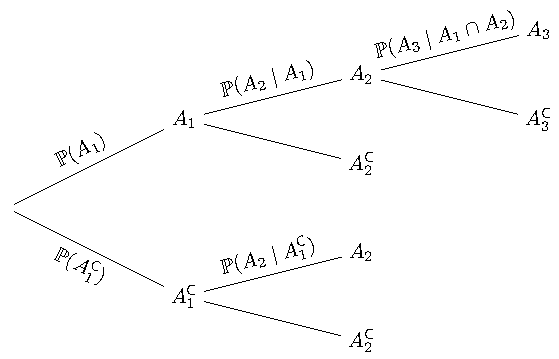
\includegraphics{./stoch_abbildungen/baum_1.pdf}
	\captionof{figure}{Darstellung eines Stufenexperiments}
\end{center}

\begin{satz}[Konstruktion des Wahrscheinlichkeitsmaßes eines Stufenexperiments] \label{satz: 3_1_6_stufenexperiment}
	Gegeben seinen $n$ Ergebnisräume $\Omega_i = \menge{\omega_i (1), \dots, \omega_i (k)}, k \in \N \cup \menge{\infty}$ und es sei $\Omega = \Omega_1 \times \cdots \Omega_n$ der zugehörige Produktraum. Weiter seinen $\F_i$ $\sigma$-Algebren auf $\Omega_i$ und $\F = \bigotimes_{i=1}^n \F_i$ die Produkt-$\sigma$-Algebra auf $\Omega$. Setze $\omega = (\omega_1,\dots,\omega_n)$ und
	\begin{equation*}
	[\omega_1,\dots,\omega_m] \defeq \menge{\omega_1}\times \dots \times \menge{\omega_m} \times \Omega_{m+1} \times \cdots \times \Omega_{n} \qquad (m \leq n) 
	\end{equation*}
	und
	\begin{equation*}
		\P(\menge{\omega_m} \mid [\omega_1,\dots,\omega_{m-1}])
	\end{equation*}
	für die Wahrscheinlichkeit in der $m$-ten Stufe des Experiments $\omega_m$ zu beobachten, falls in den vorausgehenden Stufen $\omega_1,\dots,\omega_{m-1}$ beobachten wurden. Dann definiert
	\begin{equation*}
		\P(\menge{\omega}) \defeq \P(\menge{\omega_1}) \prod_{m=2}^{n}\P\brackets{\menge{\omega_m} \mid [\omega_1, \dots, \omega_{m-1}]}
	\end{equation*}
	ein Wahrscheinlichkeitsmaß auf $(\Omega, \F, \P)$.
\end{satz}
\begin{proof}
	Nachrechnen!
\end{proof}

\begin{beispiel}[\person{Polya}-Urne]
	Gegeben sei eine Urne mit $s$ schwarzen und $w$ weißen Kugeln. Bei jedem Zug wird die  gezogene Kugel zusammen mit $c \in \N_0 \cup \menge{-1}$ weiteren Kugeln derselben Farbe zurückgelegt.
	\begin{itemize}
		\item $c=0$: Urnenmodell mit Zurücklegen
		\item $c=-1$: Urnenmodell ohne Zurücklegen
	\end{itemize}
	Beide haben wir schon in Kapitel 2.2 gesehen. 
	Sei deshalb $c\in \N$ (Bsp. Modell für zwei konkurrierende Populationen). Ziehen wir $n$-mal, so haben wir ein $n$-Stufenexperiment mit 
	\begin{equation*}
		\Omega = \menge{0,1}^n \mit \text{ 0 = ``weiß'', 1 = ``schwarz''} \quad (\Omega_i = \menge{0,1})
	\end{equation*}
	Zudem gelten im ersten Schritt
	\begin{equation*}
		\P(\menge{0}) = \frac{w}{s+w} \und \P(\menge{1}) = \frac{s}{s+w}
	\end{equation*}
	sowie
	\begin{equation*}
		\P(\menge{\omega_m} \mid [\omega_1, \dots \omega_{m-1}]) = 
		\begin{cases}
		\frac{w+c \brackets{m-1 - \sum_{i=1}^{m-1}\omega_i}}{s+w+c(m-1)} & \omega_m = 0\\
		\frac{s + c\sum_{i=1}^{m-1}\omega_i}{s+w+c(m-1)} & \omega_m = 1
		\end{cases}
	\end{equation*}
	Mit \cref{satz: 3_1_6_stufenexperiment} folgt als Wahrscheinlichkeitsmaß auf $(\Omega, \pows(\Omega))$
	\begin{equation*}
	\begin{aligned}
		\P(\menge{(\omega_1, \dots, \omega_n)}) 
		&= \P(\menge{\omega_1}) \prod_{m=2}^n \P(\menge{\omega_m}\mid [\omega_1,\dots,\omega_{m-1}]) \\
		&= \frac{\prod_{i=0}^{l-1}(s+c * i) \, \prod_{j=0}^{n-l-1}(w + c * j)}{\prod_{i=0}^n (s+w+c * i)}
	\end{aligned}
	\end{equation*}
	mit $l=\sum_{i=1}^n \omega_i$. Definiere wir nun die Zufallsvariable
	\begin{equation*}
		\abb{S_n}{\Omega}{\N_0} \mit (\omega_1, \dots, \omega_n) \mapsto \sum_{i=1}^n \omega_i
	\end{equation*}
	welche die Anzahl der gezogenen schwarzen Kugeln modelliert, so folgt
	\begin{equation*}
		\P(S_n = l) = \binom{n}{l} \frac{\prod_{i=0}^{l-1}(s+c * i) \, \prod_{j=0}^{n-l-1}(w + c * j)}{\prod_{i=0}^n(s+w+c * i)}
	\end{equation*}
	Mittels $a \defeq \lfrac{s}{c}$ und $b \defeq \lfrac{w}{c}$ folgt
	\begin{equation*}
		\begin{aligned}
			\P(S_n = l) = \binom{n}{l} \frac{\prod_{i=0}^{l-1}(-a-i)\prod_{j=0}^{n-l-1}(-b-j)}{\prod_{i=0}^n (-a-b-i)} = \frac{\binom{-a}{l}\binom{-b}{n \cdot l}}{\binom{-a-b}{n}} \mit l \in \menge{0,\dots,n} 
		\end{aligned}
	\end{equation*}
	Dies ist die \begriff{\person{Polya}-Verteilung} auf $\menge{0,\dots,n}$ ($n \in \N$) mit Parametern $a,b > 0$.
\end{beispiel}

\begin{beispiel} \label{beispiel_3_1_8_multiplechoice}
	Ein Student beantwortet eine Multiple-Choice-Frage mit vier Antwortmöglichkeiten, eine davon ist richtig. Er kennt die richtige Antwort mit Wahrscheinlichkeit $\lfrac{2}{3}$. Wenn er die richtige Antwort kennt, so wählt er diese aus. Andernfalls wählt er zufällig (gleichverteilt) eine Antwort. Betrachten wir 
	\begin{equation*}
		W = \menge{\text{richtige Antwort gewusst}} \und 
		R = \menge{\text{Richtige Antwort gewählt}}
	\end{equation*}
	Dann gilt
	\begin{equation*}
		\P(W) = \frac{2}{3} \qquad \P(R \mid W) = 1 \qquad \P(R \mid W^\complement) = \frac{1}{4}
	\end{equation*}
	Angenommen der Student gibt die richtige Antwort. Mit welcher Wahrscheinlichkeit hat er diese gewusst? $\longrightarrow \enskip \P(W \mid R) = \text{ ?}$
\end{beispiel}

\begin{satz} \label{satz: 3_1_9_totaleW_bayes}
	Sei $(\Omega, \F, \P)$ ein Wahrscheinlichkeitsraum und $\Omega = \bigcup_{i \in I} B_i$ eine höchstens abzählbare Zerlegung in paarweise disjunkte Ereignisse $B_i \in \F$.
	\begin{enumerate}
		\item \textit{Satz von der totalen Wahrscheinlichkeit:} Für alle $A \in \F$ gilt
		\begin{align}
			\P(A) = \sum_{i\in I} \P(A\mid B_i) * \P(B_i) \label{eq: totaleWkeit}
		\end{align} 
		\item \textit{Satz von \person{Bayes}:} Für alle $A \in \F$ mit $\P(A) > 0$ und alle $k \in I$ gilt
		\begin{align}
			\P(B_k \mid A) = \frac{\P(A \mid B_k) * \P(B_k)}{\sum_{i\in I}\P(A\mid B_i) * \P(B_i)} \label{eq: bayes}
		\end{align}
	\end{enumerate}
\end{satz}

\begin{proof}
	Es gilt:
	\begin{equation*}
		\sum_{i\in I} \P(A\mid B_i) * \P(B_i) = \sum_{i\in I}\frac{\P(A \cap B_i)}{\P(B_i)} * \P(B_i) = \sum_{i\in I} \P(A \cap B_i) \overset{\sigma-Add.}{=} \P(A)
	\end{equation*}
	und
	\begin{equation*}
	\P(B_k \mid A) = \frac{\P(A \cap B_k)}{\P(A)} = \frac{\P(A \mid B_k) * \P(B_k)}{\P(A)}
	\end{equation*}
	also folgt (b) aus (a).
\end{proof}

\begin{beispiel}
	In der Situation von \cref{beispiel_3_1_8_multiplechoice} folgt mit \labelcref{eq: totaleWkeit}
	\begin{equation*}
	\begin{aligned}
		\P(R) 
		&= \P(R \mid W) * \P(W) + \P(R \mid W^\complement) * \P(W^\complement) \\
		&= 1 \cdot \frac{2}{3} + \frac{1}{4} * \frac{1}{3} = \frac{3}{4}
	\end{aligned}
	\end{equation*}
	und mit \labelcref{eq: bayes}
	\begin{equation*}
		\P(W \mid R) = \frac{\P(R \mid W) * \P(W)}{\P(R)} = \frac{1 * \frac{2}{3}}{\frac{3}{4}} = \frac{8}{9}
	\end{equation*}
	für die gesuchte Wahrscheinlichkeit.
	\begin{center}
		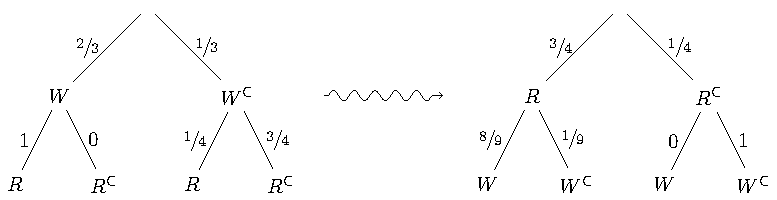
\includegraphics{./stoch_abbildungen/baum_2.pdf}
		\captionof{figure}{Bedingte Wahrscheinlichkeit im Baumdiagramm}
	\end{center}
\end{beispiel}